\documentclass[tikz,border=4pt]{standalone}
\usepackage[T1]{fontenc}
\usepackage{lmodern}
\usepackage{amsmath,amssymb}
\usetikzlibrary{arrows.meta,positioning,shapes.geometric,fit,calc,decorations.pathreplacing}

\definecolor{stageblue}{RGB}{15,70,235}
\definecolor{stagered}{RGB}{235,30,25}
\definecolor{stageorange}{RGB}{255,85,25}
\definecolor{stagegreen}{RGB}{0,120,40}
\definecolor{stagepurple}{RGB}{90,25,240}

\tikzset{
  font=\sffamily,
  arr/.style={-{Stealth[length=2.6mm,width=2.0mm]},line width=.72pt,draw=black},
  redarr/.style={-{Stealth[length=2.5mm,width=1.9mm]},line width=.72pt,draw=stagered},
  bluebox/.style={draw=stageblue,line width=.72pt,rounded corners=1.5pt,fill=white},
  orangebox/.style={draw=stageorange,line width=.72pt,rounded corners=1.5pt,fill=white},
  greenbox/.style={draw=stagegreen,line width=.72pt,rounded corners=1.5pt,fill=white},
  purplebox/.style={draw=stagepurple,line width=.72pt,rounded corners=1.5pt,fill=white},
  decision/.style={diamond,aspect=2.15,draw=black,line width=.72pt,fill=white,inner sep=1.5pt},
  dashblue/.style={draw=stageblue,dashed,line width=.72pt,rounded corners=2pt},
  dashorange/.style={draw=stageorange,dashed,line width=.72pt,rounded corners=2pt}
}

% Small editable chromosome used in the Evolution Stage.
\newcommand{\chromosome}[3]{%
  \begin{scope}[shift={(#1,#2)},scale=#3]
    \foreach \x/\c in {0/blue,0.36/cyan,0.72/blue,1.08/green,1.44/orange,1.80/red}{
      \filldraw[fill=\c!75,draw=black,line width=.25pt] (\x,0) rectangle ++(.36,.30);
      \fill[white] (\x+.15,.13) circle (.025);
    }
  \end{scope}%
}

\begin{document}
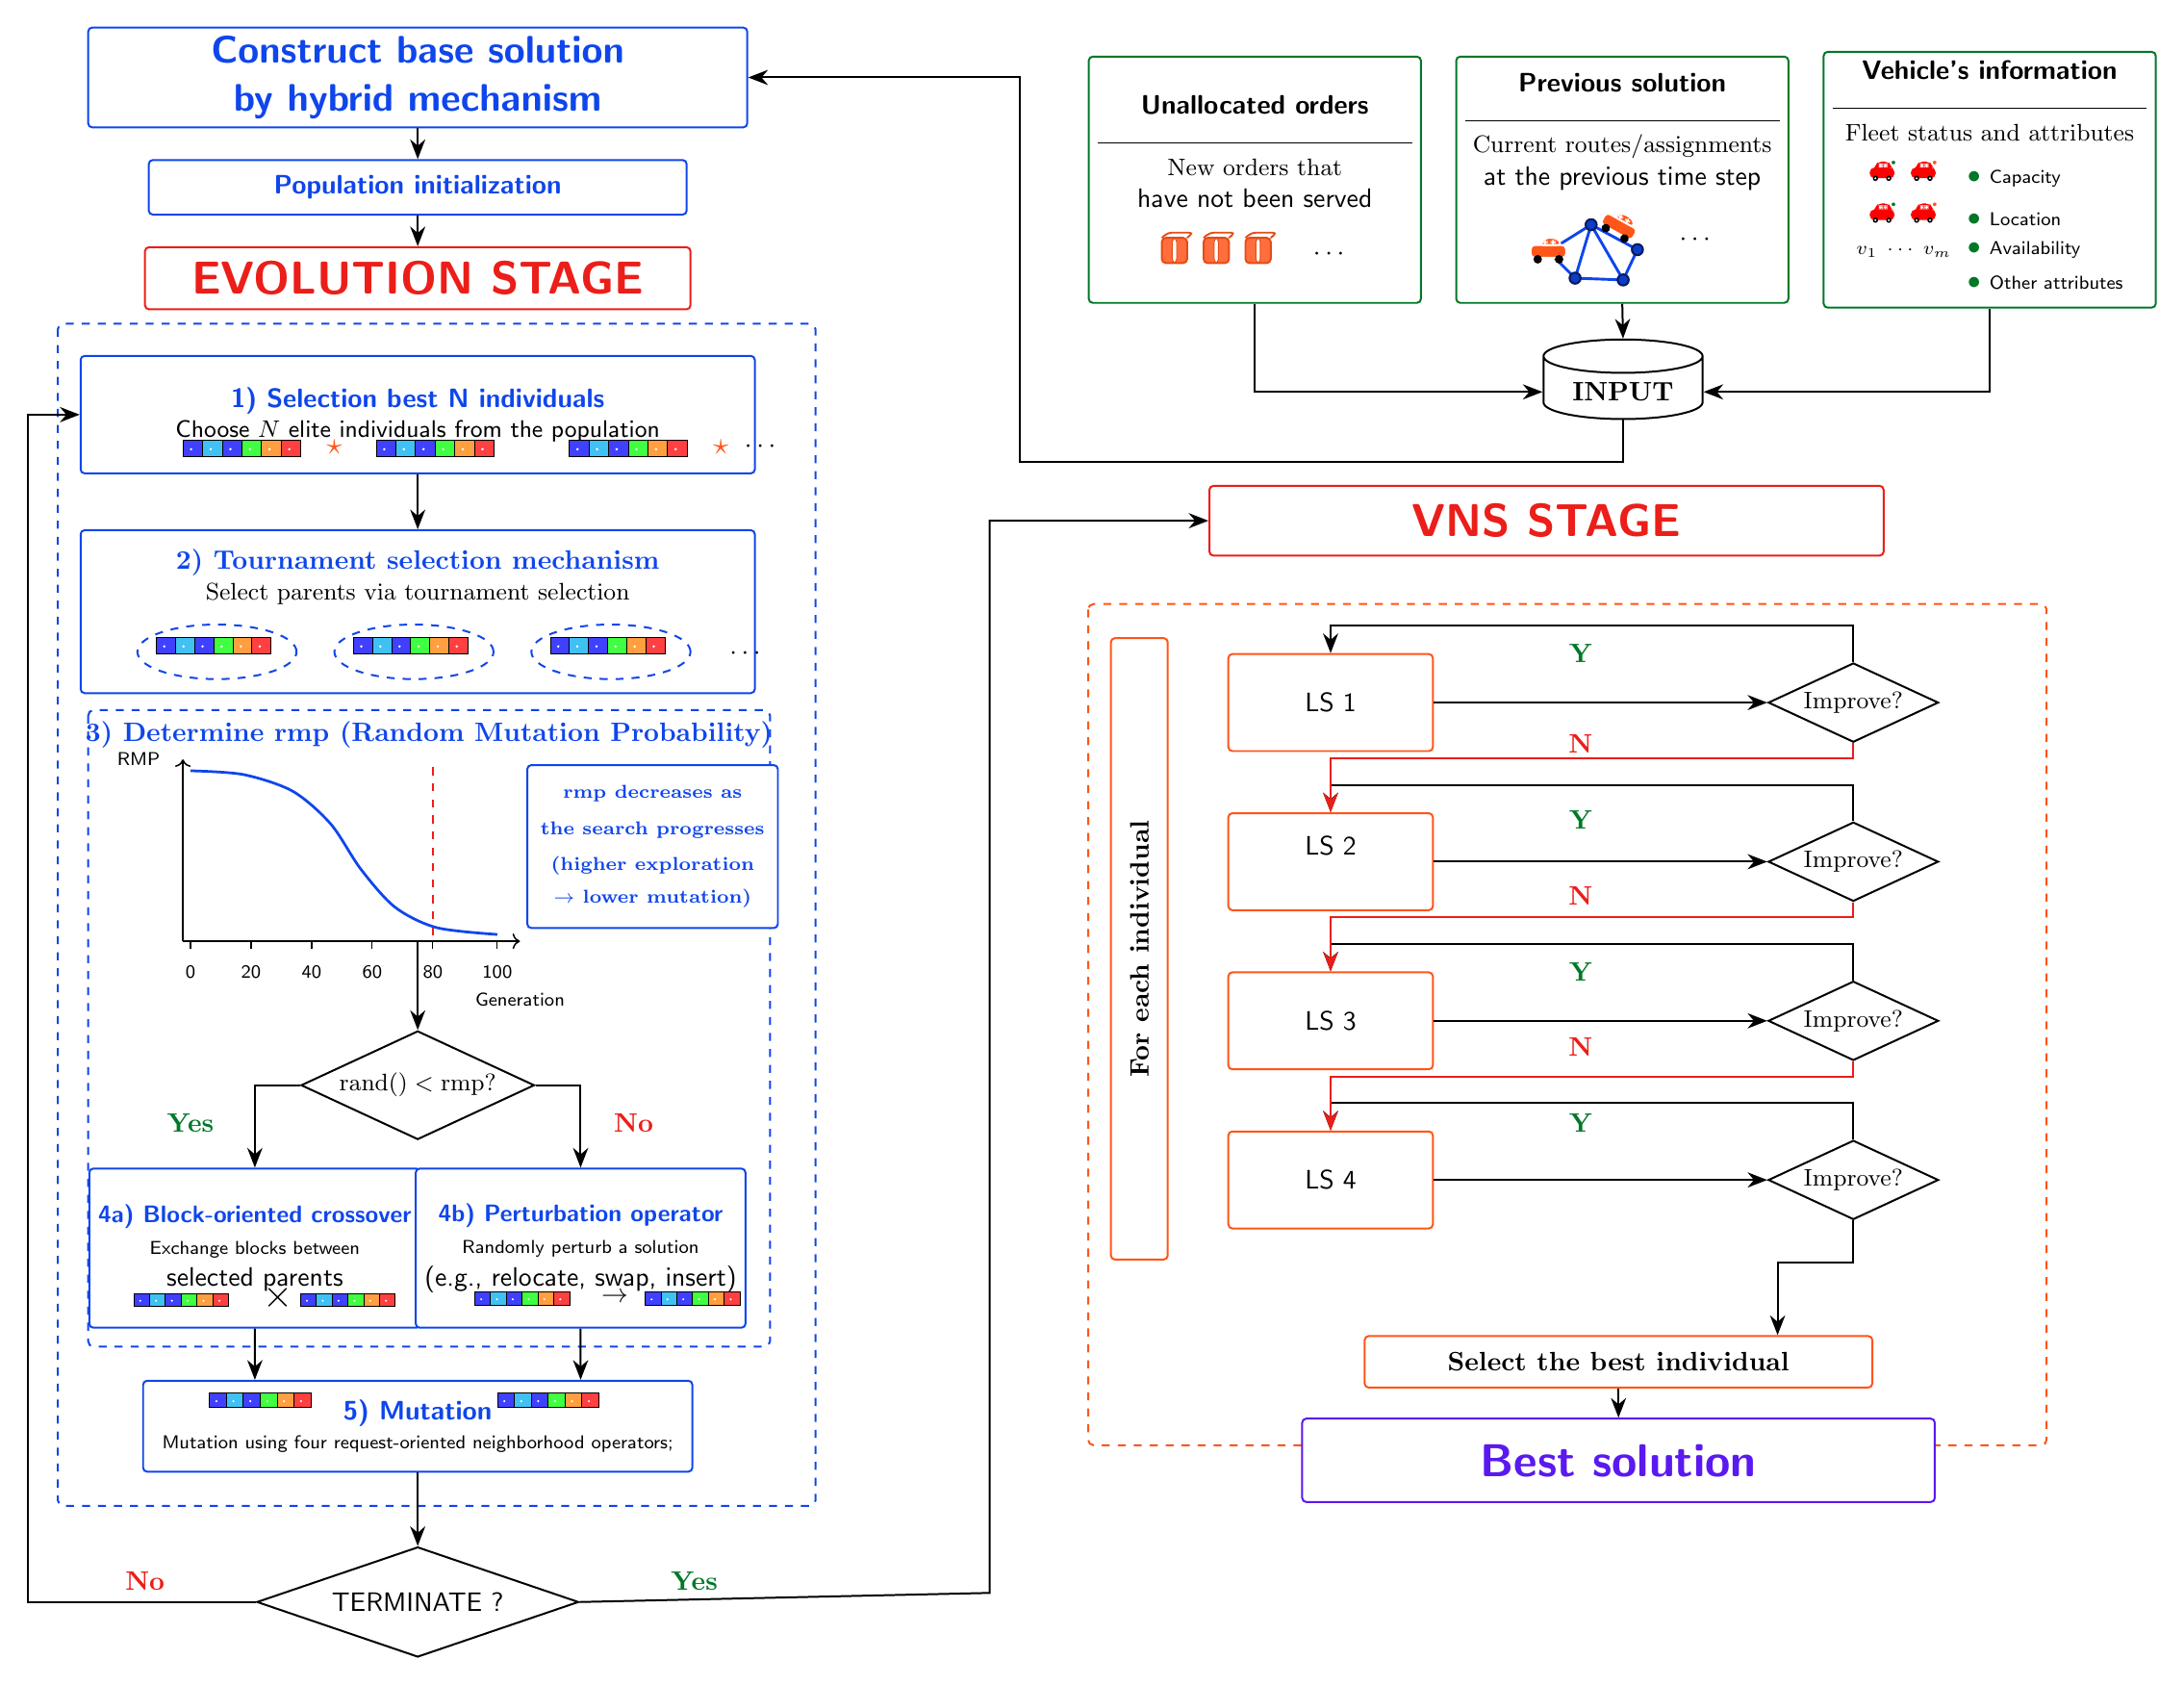
\begin{tikzpicture}[x=1cm,y=1cm]

% ------------------------------------------------------------------
% LEFT: EVOLUTION STAGE
% ------------------------------------------------------------------
\node[bluebox,minimum width=8.7cm,minimum height=1.25cm,align=center,
      text=stageblue,font=\sffamily\bfseries\Large] (construct) at (5.2,18.8)
      {Construct base solution\\by hybrid mechanism};
\node[bluebox,minimum width=7.1cm,minimum height=.72cm,
      text=stageblue,font=\sffamily\bfseries] (init) at (5.2,17.35)
      {Population initialization};
\node[draw=stagered,line width=.72pt,rounded corners=1.5pt,
      minimum width=7.2cm,minimum height=.82cm,
      text=stagered,font=\sffamily\bfseries\LARGE] (etitle) at (5.2,16.15)
      {EVOLUTION STAGE};
\draw[arr] (construct)--(init);
\draw[arr] (init)--(etitle);

\coordinate (EtopL) at (.45,15.55);
\coordinate (EbotR) at (10.45,-.05);
\draw[dashblue] (EtopL) rectangle (EbotR);

\node[bluebox,minimum width=8.9cm,minimum height=1.55cm,align=center] (sel) at (5.2,14.35)
 {\textcolor{stageblue}{\bfseries 1) Selection best N individuals}\\[-1pt]
  {\small Choose $N$ elite individuals from the population}};
\chromosome{2.1}{13.80}{.72}
\chromosome{4.65}{13.80}{.72}
\chromosome{7.20}{13.80}{.72}
\node[text=stageorange,font=\large] at (4.10,13.92) {$\star$};
\node[text=stageorange,font=\large] at (9.20,13.92) {$\star$};
\node at (9.75,13.92) {$\cdots$};

% Khung bao ngoài
% Toàn bộ phần này lùi xuống 0.5 cm
\begin{scope}[yshift=-0.5cm]

\node[
  bluebox,
  minimum width=8.9cm,
  minimum height=2.15cm
] (tour) at (5.2,12.25) {};

% Tiêu đề
\node[
  text=stageblue,
  font=\bfseries
] at (5.2,12.90)
{2) Tournament selection mechanism};

% Phần mô tả
\node[
  font=\small
] at (5.2,12.48)
{Select parents via tournament selection};

% Các chromosome
\chromosome{1.75}{11.70}{.70}
\chromosome{4.35}{11.70}{.70}
\chromosome{6.95}{11.70}{.70}

% Các đường ellipse bao quanh chromosome
\draw[dashblue]
  (2.55,11.72) ellipse (1.05cm and .36cm);

\draw[dashblue]
  (5.15,11.72) ellipse (1.05cm and .36cm);

\draw[dashblue]
  (7.75,11.72) ellipse (1.05cm and .36cm);

% Ký hiệu so sánh
\node at (4.00,11.70) {\small };
\node at (6.60,11.70) {\small };
\node at (9.55,11.70) {$\cdots$};

% Khung khối số 3
\draw[dashblue]
  (.85,10.95) rectangle (9.85,2.55);

\node[
  text=stageblue,
  font=\bfseries
] at (5.35,10.63)
{3) Determine rmp (Random Mutation Probability)};

% Trục Generation
\draw[
  ->,
  line width=.55pt
]
  (2.10,7.90)--(6.55,7.90)
  node[below=16pt] {\scriptsize Generation};

% Trục RMP
\draw[
  ->,
  line width=.55pt
]
  (2.10,7.90)--(2.10,10.30)
  node[left=5pt] {\scriptsize RMP};

% Đường biểu diễn RMP
\draw[
  stageblue,
  line width=1.0pt
]
  plot[smooth] coordinates {
    (2.20,10.15)
    (2.90,10.10)
    (3.55,9.88)
    (4.05,9.45)
    (4.45,8.85)
    (4.90,8.35)
    (5.45,8.08)
    (6.25,7.99)
  };

% Các mốc trên trục Generation
\foreach \x/\t in {
  2.20/0,
  3.00/20,
  3.80/40,
  4.60/60,
  5.40/80,
  6.25/100
}{
  \draw
    (\x,7.90)--++(0,-.10)
    node[below=3pt] {\scriptsize \t};
}



% Vẽ bên ngoài scope để nối đúng hai khối
\draw[arr] (sel)--(tour);

\node[
  bluebox,
  minimum width=2.80cm,
  minimum height=2.15cm,
  inner xsep=5pt,
  inner ysep=6pt,
  align=center,
  text=stageblue,
  font=\scriptsize\bfseries
] at (8.30,9.15)
{
  rmp decreases as\\[2mm]
  the search progresses\\[2mm]
  (higher exploration\\[1.5mm]
  $\rightarrow$ lower mutation)
};

% Đường nét đứt tại thế hệ 80
\draw[
  stagered,
  dashed,
  line width=.6pt
]
  (5.40,7.98)--(5.40,10.25);

% Hạ khối hình thoi xuống để tạo khoảng cách với đồ thị
\node[
  decision,
  minimum width=1.65cm,
  minimum height=0.70cm,
  font=\small
] (rand) at (5.20,6.0)
  {$\operatorname{rand()} < \operatorname{rmp}?$};

% Mũi tên nối từ đồ thị xuống hình thoi

\draw[arr]
  (5.20,7.90)--(rand.north);
  
% Nhãn Yes/No
% y: 7.00 → 5.50
\node[text=stagegreen,font=\bfseries]
  at (2.20,5.50) {Yes};

\node[text=stagered,font=\bfseries]
  at (8.05,5.50) {No};

% Khối crossover và perturbation
% y: 5.35 → 3.85
\node[
  bluebox,
  minimum width=4.05cm,
  minimum height=2.10cm,
  align=center
] (cross) at (3.05,3.85)
{
  \textcolor{stageblue}{\bfseries\small
  4a) Block-oriented crossover}\\
  \scriptsize
  Exchange blocks between\\
  selected parents
};

\node[
  bluebox,
  minimum width=4.05cm,
  minimum height=2.10cm,
  align=center
] (pert) at (7.35,3.85)
{
  \textcolor{stageblue}{\bfseries\small
  4b) Perturbation operator}\\
  \scriptsize
  Randomly perturb a solution\\
  (e.g., relocate, swap, insert)
};

% Hình minh họa trong hai khối
% y: 4.58 → 3.08
\chromosome{1.45}{3.08}{.58}
\chromosome{3.65}{3.08}{.58}

% y: 4.70 → 3.20
\node[font=\Large] at (3.35,3.20) {$\times$};

% y: 4.60 → 3.10
\chromosome{5.95}{3.10}{.58}

% y: 4.70 → 3.20
\node at (7.80,3.20) {$\rightarrow$};

\chromosome{8.2}{3.10}{.58}

% Mũi tên từ rand đến hai khối
\draw[arr] (rand.west)-|(cross.north);
\draw[arr] (rand.east)-|(pert.north);

% Khối Mutation
% y: 3.65 → 2.15
\node[
  bluebox,
  minimum width=7.25cm,
  minimum height=1.20cm,
  align=center
] (mut) at (5.20,1.5)
{
  \textcolor{stageblue}{\bfseries
  5) Mutation}\\[-1pt]
  {\scriptsize Mutation using four request-oriented neighborhood operators;}
};

% Hình minh họa Mutation
% y: 3.25 → 1.75
\chromosome{2.45}{1.75}{.62}
\chromosome{6.25}{1.75}{.62}

% y: 3.36 → 1.86

% Mũi tên xuống Mutation
% Mũi tên thẳng từ cross xuống Mutation
\draw[arr]
  (cross.south)
  --($(mut.north)+(-2.15,0)$);

% Mũi tên thẳng từ pert xuống Mutation
\draw[arr]
  (pert.south)
  --($(mut.north)+(2.15,0)$);

% Khối TERMINATE
% y: 0.68 → -0.82
\node[
  decision,
  minimum width=4.25cm,
  minimum height=.92cm
] (term) at (5.20,-0.82)
  {TERMINATE ?};

\draw[arr] (mut)--(term);

% Nhãn No và Yes
% y: 0.95 → -0.55
\node[text=stagered,font=\bfseries]
  at (1.60,-0.55) {No};

\node[text=stagegreen,font=\bfseries]
  at (8.85,-0.55) {Yes};

% Nhánh quay lại Selection
\draw[arr]
  (term.west)
  --(.05,-0.82)
  --(.05,14.85)
  --(sel.west);
\end{scope}
% ------------------------------------------------------------------
% TOP-RIGHT: INPUT DATA
% ------------------------------------------------------------------
\node[
  greenbox,
  minimum width=4.2cm,
  minimum height=3.25cm,
  align=center
] (orders) at (16.25,17.45)
{
  \bfseries Unallocated orders\\[-1pt]
  \rule{4.15cm}{.35pt}\\
  \normalfont\small
  New orders that\\
  have not been served\\[8pt]
  \raisebox{-1pt}{%
    \tikz[scale=0.23,baseline]{
      \foreach \x in {0,2.4,4.8}{
        \filldraw[
          fill=stageorange!85,
          draw=stageorange!90!black,
          line width=.7pt
        ]
          (\x,0) rectangle ++(1.45,1.45);

        \draw[
          stageorange!90!black,
          line width=.7pt
        ]
          (\x,1.45)
          --++(.35,.30)
          --++(1.45,0)
          --++(-.35,-.30);

        \filldraw[
          fill=white!85,
          draw=stageorange!90!black,
          line width=.35pt
        ]
          (\x+.60,0) rectangle ++(.25,1.45);
      }
    }%
  }
  \quad$\cdots$
};
\node[
  greenbox,
  minimum width=4.2cm,
  minimum height=3.25cm,
  align=center
] (prev) at (21.10,17.45)
{
  \bfseries Previous solution\\[-1pt]
  \rule{4.15cm}{.35pt}\\
  \normalfont\small
  Current routes/assignments\\
  at the previous time step\\[7pt]

  \raisebox{-2pt}{%
    \tikz[
      scale=.47,
      line cap=round,
      line join=round,
      baseline
    ]{
      % Các cạnh của đồ thị
      \draw[
        stageblue,
        line width=1.05pt
      ]
        (0,0)
        --(1.20,.75)
        --(2.50,.05)
        --(2.10,-.80)
        --(.75,-.75)
        --(0,0);

      \draw[
        stageblue,
        line width=1.05pt
      ]
        (1.20,.75)--(.75,-.75);

      \draw[
        stageblue,
        line width=1.05pt
      ]
        (1.20,.75)--(2.10,-.80);

      % Các đỉnh: tăng kích thước và độ đậm
      \foreach \x/\y in {
        0/0,
        1.20/.75,
        2.50/.05,
        2.10/-.80,
        .75/-.75
      }{
        \filldraw[
          fill=stageblue!85!black,
          draw=stageblue!40!black,
          line width=.75pt
        ]
          (\x,\y) circle (.155);
      }

      % Ô tô thứ nhất:
      % đặt lệch phía trên cạnh để không đè lên đường
      \begin{scope}[scale=2,transform shape]
        shift={(.60,.65)},
        rotate=32
      ]
        % Viền trắng giúp ô tô tách khỏi đồ thị
        \filldraw[
          fill=stageorange,
          draw=white,
          line width=.75pt
        ]
          (-.25,-.09) rectangle (.25,.09);

        \filldraw[
          fill=stageorange,
          draw=white,
          line width=.65pt
        ]
          (-.13,.09)
          --(-.05,.19)
          --(.12,.19)
          --(.19,.09)
          --cycle;

        % Cửa kính
        \fill[white]
          (-.08,.10) rectangle (-.01,.16);

        \fill[white]
          (.03,.10) rectangle (.10,.16);

        % Bánh xe
        \fill[black] (-.15,-.11) circle (.06);
        \fill[black]  (.15,-.11) circle (.06);
      \end{scope}

      % Ô tô thứ hai:
      % đặt lệch phía trên cạnh bên phải
      % Ô tô thứ hai
\begin{scope}[
  shift={(1.98,.70)},
  rotate=-29
]
  % Phóng to riêng ô tô, không làm thay đổi vị trí
  \begin{scope}[scale=2]

    % Thân xe
    \filldraw[
      fill=stageorange,
      draw=white,
      line width=.75pt
    ]
      (-.25,-.09) rectangle (.25,.09);

    % Mui xe
    \filldraw[
      fill=stageorange,
      draw=white,
      line width=.65pt
    ]
      (-.13,.09)
      --(-.05,.19)
      --(.12,.19)
      --(.19,.09)
      --cycle;

    % Hai cửa kính
    \fill[white]
      (-.08,.10) rectangle (-.01,.16);

    \fill[white]
      (.03,.10) rectangle (.10,.16);

    % Hai bánh xe
    \fill[black]
      (-.15,-.11) circle (.06);

    \fill[black]
      (.15,-.11) circle (.06);

  \end{scope} % kết thúc scope phóng to
\end{scope}   % kết thúc scope định vị và xoay
    }%
  }
  \quad$\cdots$
};


  
% \node[greenbox,minimum width=4.2cm,minimum height=3.25cm,align=center] (vehicle) at (25.95,17.45)
%  {\bfseries Vehicle's information\\[-1pt]\rule{4.15cm}{.35pt}\\
%   \normalfont\small Fleet status and attributes\\[6pt]
%   $v_1\ \cdots\ v_m$\qquad
%   \shortstack[l]{\scriptsize Capacity\\\scriptsize Location\\\scriptsize Availability\\\scriptsize Other attributes}};

% Biểu tượng phương tiện
% Tham số #1 là màu trạng thái: stagegreen hoặc stageorange
\newcommand{\fleetcar}[1]{%
  \tikz[baseline=-0.5ex,scale=.22]{
    % Thân xe
    \filldraw[
      fill=red,
      draw=red,
      line width=.5pt
    ]
      (0,0) rectangle (1.40,.55);

    % Mui xe
    \filldraw[
      fill=red,
      draw=red,
      line width=.5pt
    ]
      (.25,.55)
      --(.48,.92)
      --(1.05,.92)
      --(1.28,.55)
      --cycle;

    % Kính xe
    \fill[white]
      (.51,.61) rectangle (.72,.84);

    \fill[white]
      (.78,.61) rectangle (1.01,.84);

    % Bánh xe
    \fill[black] (.30,-.05) circle (.16);
    \fill[white] (.30,-.05) circle (.065);

    \fill[black] (1.10,-.05) circle (.16);
    \fill[white] (1.10,-.05) circle (.065);

    % Chấm trạng thái
    \filldraw[
      fill=#1,
      draw=white,
      line width=.5pt
    ]
      (1.38,.90) circle (.16);
  }%
}

\node[
  greenbox,
  minimum width=4.2cm,
  minimum height=3.25cm,
  align=center
] (vehicle) at (25.95,17.45)
{
  \bfseries Vehicle's information\\[-1pt]
  \rule{4.15cm}{.35pt}\\
  \normalfont\small
  Fleet status and attributes\\[6pt]

  \begin{tabular}{c@{\hspace{6pt}}l}
    % Đội xe
    \fleetcar{stagegreen}\hspace{2pt}
    \fleetcar{stageorange}
    &
    \textcolor{stagegreen}{\(\bullet\)}
    {\scriptsize Capacity}
    \\[3pt]

    \fleetcar{stagegreen}\hspace{2pt}
    \fleetcar{stageorange}
    &
    \textcolor{stagegreen}{\(\bullet\)}
    {\scriptsize Location}
    \\[-1pt]

    {\scriptsize $v_1\;\cdots\;v_m$}
    &
    \textcolor{stagegreen}{\(\bullet\)}
    {\scriptsize Availability}
    \\[1pt]

    {}
    &
    \textcolor{stagegreen}{\(\bullet\)}
    {\scriptsize Other attributes}
  \end{tabular}
};


\node[draw=black,line width=.72pt,cylinder,shape border rotate=90,aspect=.28,
      minimum width=2.1cm,minimum height=1.05cm,font=\bfseries] (input) at (21.11,14.65) {INPUT};
% Unallocated orders → INPUT
\draw[arr]
  (orders.south)|-(input.west);

% Previous solution → INPUT
\draw[arr]
  (prev.south)--(input.north);

% Vehicle's information → INPUT
\draw[arr]
  (vehicle.south)|-(input.east);
\draw[arr]
  (input.south)
  --($(input.south)+(0,-0.55)$)
  -|(13.15,18.80)
  --(construct.east);

% ------------------------------------------------------------------
% RIGHT: VNS STAGE
% ------------------------------------------------------------------
\node[draw=stagered,line width=.72pt,rounded corners=1.5pt,
      minimum width=8.9cm,minimum height=.92cm,
      text=stagered,font=\sffamily\bfseries\LARGE] (vtitle) at (20.10,12.95) {VNS STAGE};
% Chuyển cá thể tốt từ Evolution Stage sang VNS Stage:
% mũi tên bắt đầu trực tiếp tại khối TERMINATE và kết thúc tại VNS STAGE.
\draw[arr]
  (term.east)
  --(12.75,-1.2)
  --(12.75,12.95)
  --(vtitle.west);
\draw[dashorange] (14.05,11.85) rectangle (26.70,.75);
\draw[draw=stageorange,line width=.72pt,rounded corners=1.5pt]
  (14.35,3.20) rectangle (15.10,11.40);
\node[rotate=90,font=\bfseries] at (14.725,7.30) {For each individual};

\node[orangebox,minimum width=2.70cm,minimum height=1.28cm,align=center] (ls1) at (17.25,10.55)
  {LS 1};
\node[decision,minimum width=2.05cm,minimum height=1.02cm,font=\small] (imp1) at (24.15,10.55) {Improve?};
\draw[arr] (ls1.east)--(imp1.west);
\draw[arr] (imp1.north)--++(0,.48)-|(ls1.north);
\node[text=stagegreen,font=\bfseries] at (20.55,11.2) {Y};

\node[orangebox,minimum width=2.70cm,minimum height=1.28cm,align=center] (ls2) at (17.25,8.45)
  {LS 2\\};
\node[decision,minimum width=2.05cm,minimum height=1.02cm,font=\small] (imp2) at (24.15,8.45) {Improve?};
\draw[arr] (ls2.east)--(imp2.west);
\draw[arr] (imp2.north)--++(0,.48)-|(ls2.north);
\node[text=stagegreen,font=\bfseries] at (20.55,9) {Y};

\node[orangebox,minimum width=2.70cm,minimum height=1.28cm,align=center] (ls3) at (17.25,6.35)
  {LS 3};
\node[decision,minimum width=2.05cm,minimum height=1.02cm,font=\small] (imp3) at (24.15,6.35) {Improve?};
\draw[arr] (ls3.east)--(imp3.west);
\draw[arr] (imp3.north)--++(0,.48)-|(ls3.north);
\node[text=stagegreen,font=\bfseries] at (20.55,7) {Y};

\node[orangebox,minimum width=2.70cm,minimum height=1.28cm,align=center] (ls4) at (17.25,4.25)
  {LS 4};
\node[decision,minimum width=2.05cm,minimum height=1.02cm,font=\small] (imp4) at (24.15,4.25) {Improve?};
\draw[arr] (ls4.east)--(imp4.west);
\draw[arr] (imp4.north)--++(0,.48)-|(ls4.north);
\node[text=stagegreen,font=\bfseries] at (20.55,5) {Y};

\draw[redarr] (imp1.south)--++(0,-.2)-|(ls2.north);
\draw[redarr] (imp2.south)--++(0,-.2)-|(ls3.north);
\draw[redarr] (imp3.south)--++(0,-.2)-|(ls4.north);
\node[text=stagered,font=\bfseries] at (20.55,10.00) {N};
\node[text=stagered,font=\bfseries] at (20.55,8) {N};
\node[text=stagered,font=\bfseries] at (20.55,6) {N};

\node[orangebox,minimum width=6.70cm,minimum height=.68cm,font=\bfseries] (choosebest) at (21.05,1.85)
 {Select the best individual};
\node[purplebox,minimum width=8.35cm,minimum height=1.10cm,
      text=stagepurple,font=\sffamily\bfseries\LARGE] (best) at (21.05,.55) {Best solution};
\draw[arr] (imp4.south)--++(0,-.55)-|($(choosebest.north)+(2.1,0)$);
\draw[arr] (choosebest)--(best);

\end{tikzpicture}
\end{document}